%%%%%%%%%%%%%%%%%%%%%%%%%%%%%%%%%%%%%%%%%%%%%%%%%%%%%%%%%%
%
% Doctoral Thesis Template @ The University of Manchester
% LaTeX Chapter Template
% Version 1 (23/07/2020)
% Joe Crone
%
% This template is based on:
% The University of Manchester, Presentation of Thesis Policy
% Research Office Graduate Education Team
% June 2017
% http://www.regulations.manchester.ac.uk/pgr-presentation-theses/
%
%%%%%%%%%%%%%%%%%%%%%%%%%%%%%%%%%%%%%%%%%%%%%%%%%%%%%%%%%%
\documentclass[../main.tex]{subfiles}
\begin{document}

% Title
%--------------------------------------------------------
\chapter{DIANA Inverse Compton Source Design}
\label{DIANA_Inverse_Compton_Source_Design} % to reference use \ref{ChapterTemplate}

\section{The DIANA Energy Recovery Linac and it's Motivation}

DIANA, the Daresbury Industrial Accelerator for Nuclear Physics Applications is an applications centric conceptual 3-turn superconducting RF ERL designed for electron based light source operations. Tunability of this light source is paramount, enabling a variety of applications from lithography to nuclear photonics and security. The DIANA ERL is anticipated to provide a high brilliance electron beam at a maximum energy of $\sim$1~\si{\giga\electronvolt} with small relative energy spread ($< 10^{-4}$) and transverse emittance ($< 1$~\si{\milli\meter}-\si{\milli\radian}) pushing the average beam current to the 10's~\si{\milli\ampere} frontier -- at the state-of-the-art for SRF ERL development. The project remains in an early conceptual phase; potential configurations for the machine and its applications are being investigated from a design choices standpoint and a user community, with scope across nuclear, particle, medical physics and material science, is being assembled.  

The ERL will be designed using a dual linac approach, with an SRF linac placed in each straight of the racetrack style configuration. The DIANA SRF linacs may either be asymmetric or symmetric; subject to a full conceptual design process. Because DIANA is a 3-turn ERL with dual linacs, a total of 6 nominal energy electron bunches must be transported through the ERL recirculation beamlines in both accelerating and decelerating configurations. A drawing of the DIANA ERL is shown in Fig.~\ref{fig:DIANA_ERL_diagram} \textcolor{blue}{**outdated diagram as placeholder**}. Currently, separate transport optics - in which the accelerating and decelerating configuration  of an electron bunch of each nominal energy has a dedicated transport beamline - is under consideration. Separate transport is selected because it offers advantages towards a multi-colour light source facility with additional control over optics in each pass at the cost of more magnets and more challenging linac entrance and exit design. A more robust analysis and justification of these design choices is presented in Section~\ref{sec:DIANA_transport_optics_investigation}. 
\begin{figure}[!h]
\centering
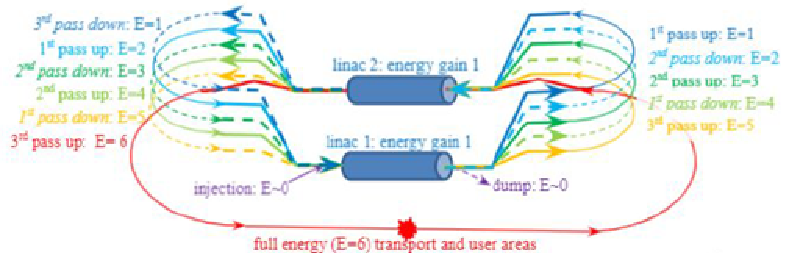
\includegraphics[width=0.8\textwidth]{Figures/DIANA_Inverse_Compton_Source_Design/DIANA_diagram_placeholder.pdf}
\caption{Drawing of the 3-turn DIANA ERL \textcolor{blue}{**PLACEHOLDER**}}
\label{fig:DIANA_ERL_diagram}
\end{figure}
Within the context of the wider accelerator community, this would be a national scale facility and is aligned to two projects in particular: a proposal for the UK-XFEL \cite{burnett2020uk} and as a solution for the Large Hadron--electron Collider (LHeC) \cite{valloni2013strawman,bruning2019exploring,holzer2021accelerator}. Within the wealth of accelerator solutions to a UK x-ray free electron laser presented in the UK-XFEL science case \cite{burnett2020uk}, a partial ERL solution is suggested with an ICS source. The UK-XFEL ICS source work is a precursor to the DIANA ICS source design as DIANA could be a potential demonstrator for the UK-XFEL. In terms of the LHeC project, the DIANA ERL could act as a proof-of-principle for the LHeC ERL alongside the existing PERLE accelerator \cite{angal2018perle}, demonstrating another design and transport approach.

High brilliance electron beams on the \si{\giga\electronvolt}-scale can facilitate applications such as a high power extreme ultraviolet (EUV) FEL and a $\gamma$-ray inverse Compton scattering source. Tunability within the electron bunch energy of the ERL is necessary for many light source experiements and must be central to the design philosophy of DIANA for useful operation of the ICS source and EUV FEL. An EUV FEL source would have far-reaching consequences for semiconductor lithography providing an unparalleled source of 13.5~\si{\nano\meter} EUV radiation (or some harmonic thereof). Whereas a high flux, narrowband  $\gamma$-ray inverse Compton scattering source driven by an ERL would have considerable impact upon nuclear physics and security, beyond the achievements and opportunities available at storage ring facilities such as HI$\gamma$S \cite{weller2009research}. Within the scope of the authors current work, the focus is on the development of the latter application as well a progress toward a conceptual design of the DIANA ERL. Hence, the following chapter excludes EUV FEL developments.

The DIANA ICS source will be driven by the ERL electron bunch, with interaction points designed directly into the transport optics, unlike in the CBETA ICS, to produce a multi-colour $\gamma$-ray source taking advantage of the three nominal energies of the DIANA ERL. A high average power 4-mirror Fabry-Perot optical re-circulation cavity is intended to store the laser pulse and interact this at a high duty factor, producing a high flux and making use of the re-circulated nature of an electron bunch in an ERL. A variable aperture circular collimator placed 10~\si{\meter} from the interaction point will then select the user-desired portion of the spectral output for narrowband operation, making use of the energy--angle correspondence  Through specification of the ERL with a focus toward $\gamma$-ray production and design of the interaction points using optimisation procedures developed in Chapter~\ref{Optimisation_and_Characterisation_of_Inverse_Compton Scattering_Spectra}, the DIANA ICS source aims to produce narrowband ($< 1$\% \textit{rms} BW) radiation on the \si{\mega\electronvolt}-scale. 

A $\gamma$-ray ICS source at moderate energies ($E_{\gamma} < 5$~\si{\mega\electronvolt}) could enable applications such as nuclear resonance fluorescence (NRF) for inspection of nuclear fuel rods, waste studies and detection of clandestine nuclear material \cite{angell2015demonstration,bolind2015states} to high energy ($E_{\gamma} > 5$~\si{\mega\electronvolt}) applications such as nuclear photonics \cite{budker2021expanding} and medical isotope production \cite{habs2011production}. The scattered photon energy regime of nuclear photonics lays in the $\sim$20~\si{\mega\electronvolt} regime and above - at the limitations in energy of the DIANA ICS source. However, the scattered photon energy of the DIANA ICS can be extended to $\sim$40~\si{\mega\electronvolt} through use of frequency doubled lasers such as the commonly used 2nd harmonic of a Nd:YAG ($\lambda =$532~\si{\nano\meter}) laser \cite{} \textcolor{blue}{**WHO SUGGESTS THIS?**}. Within the applications of a DIANA ERL driven ICS source, special consideration is given to the photo-nuclear production of medical isotopes. 

\section{Transport Optics Investigation}
\label{sec:DIANA_transport_optics_investigation}

\section{ERL ICS Electron Beam and Optical Cavity Laser Pulse Parameters}
\subsection{ERL ICS Electron Beam Parameters }
The electron bunch parameters for the DIANA ERL ICS are presented in Table~\ref{tab:DIANA_electron_beam_design_parameters}. The DIANA electron bunch parameters target a high brilliance electron bunch for operation of a high quality ICS and FEL light source facility. The focus of the parameter set displayed here is on maximising the ICS output, however these parameters are broadly applicable to development of a high brilliance FEL, with some adjustment to the longitudinal parameters resulting from the necessity of coherence in FELs requiring short bunch lengths and high peak powers.    

\begin{table}[!h]
\centering
\caption{Electron beam parameters foreseen at the DIANA ICS source interaction point (IP). Baseline parameters assume a round transverse profile for the electron bunch whereas the optimised parameters are the result of a simplex non-round beam optimisation. The given baseline parameters -- which assume the same $\beta^*$ at the IP -- allow a comparison of flux and bandwidth at different energies. The optimised values beneath those are designed to maximise the flux into a 0.5\% \textit{rms} scattered photon bandwidth through a trade-off of $\beta$-function of the electron bunch in each transverse plane and collimation angle.}
\vspace{3mm}
\begin{threeparttable}
\begin{tabular}{lccccc}
\hline\hline
Parameter & \multicolumn{3}{c}{Quantity} & Unit \\
\hline
Turn number & 1 & 2 & 3  \\
Injection Energy, $E_{\mathrm{inj}}$ & \multicolumn{3}{c}{7} & \si{\mega\electronvolt}\\
\tnote{$\dagger$}~Electron kinetic energy, $E_e$ & 362 & 717 & 1072 & \si{\mega\electronvolt}\\
Harmonic Frequency, $f$ & \multicolumn{3}{c}{125} & \si{\mega\hertz}\\
Bunch charge, $e N_e$ & \multicolumn{3}{c}{100} & \si{\pico\coulomb} \\
Avg. beam current, $I$ & \multicolumn{3}{c}{12.5} & \si{\milli\ampere} \\
Transverse normalised \textit{rms} emittance, $\epsilon_{N}$ & \multicolumn{3}{c}{0.5} & \si{\milli\meter}-\si{\milli\radian}\\
\tnote{$\sharp$}~\textit{rms} bunch length, $\Delta \tau$ & \multicolumn{3}{c}{0.9 (3)} & \si{\milli\meter} (\si{\pico\second})\\
Bunch spacing, $t_{b}$ & \multicolumn{3}{c}{8} & \si{\nano\second} \\
RF frequency, $f_{RF}$ & \multicolumn{3}{c}{750} & \si{\mega\hertz} \\
\tnote{*}~Absolute energy spread, $\Delta E_{e}$ & \multicolumn{3}{c}{$\sim$10} & \si{\kilo\electronvolt} \\ 
\tnote{*}~Relative energy spread, $\left(\Delta E_{e}/E_{e}\right)$ & \multicolumn{3}{c}{$\sim10^{-5}$} & \\
\hline
\multicolumn{5}{c}{Baseline Parameters} \\
\hline
$\beta$-functions at the IP, $\beta_{x}^{*}$/$\beta_{y}^{*}$ & 0.2/0.2 & 0.2/0.2 & 0.2/0.2 & \si{\meter} \\
Electron bunch spot size, $\sigma_{e,x}$/$\sigma_{e,y}$ & 11.87/11.87 & 8.44/8.44 & 6.90/6.90 & \si{\micro\meter}\\
\hline\multicolumn{5}{c}{Optimised 0.5\% \textit{rms} Bandwidth} \\
\hline
$\beta$-functions at the IP $\beta_{x}^{*}$/$\beta_{y}^{*}$ & 1.33/0.298 & 2.62/0.587 & 3.90/0.874 & \si{\meter} \\
Electron bunch spot size, $\sigma_{e,x}$/$\sigma_{e,y}$ & 30.62/14.49 & 30.54/14.46 & 30.48/14.43 & \si{\micro\meter}\\
Collimation Angle, $\theta_{\mathrm{col}}$ & 0.180 & 0.091 & 0.061 & \si{\milli\radian} \\ 
\hline\hline
\end{tabular}
\begin{tablenotes}
\item[$\sharp$]{Taken from the ASML parameters.}
\item[*]{Estimated values.}
\item[$\dagger$]{Electron beam energies to accomplish $E_{\gamma}^{\mathrm{max}}$ = 20~\si{\mega\electronvolt} $\gamma$-rays. $\Delta E_{\mathrm{turn}}$ = 355~\si{\mega\electronvolt}.}
\end{tablenotes}
\end{threeparttable}
\label{tab:DIANA_electron_beam_design_parameters}
\end{table}

Baseline parameters are designed in order to maximise the uncollimated flux and brilliance of the ICS source. Therefore, the case of a small interaction point $\beta$-function, which is kept constant, is used to produce a small electron spot size at the IP. The constant $\beta$-function in the baseline case is also useful for highlighting changes within the spectral output that characterises source performance, allowing effects due to the varying kinetic energy of the electron bunch to be disentangled. A non-round beam optimised case is also shown for maximising the collimated flux into a narrow 0.5\% bandwidth, which is optimised using the simplex non-round beam methodology in Chapter~\ref{Optimisation_and_Characterisation_of_Inverse_Compton Scattering_Spectra}. The 0.5\% optimised \textit{rms} bandwidth case is designed to show the ability of DIANA to produce high flux into a narrow bandwidth, required by some nuclear physics experiments, and investigate the difference between ICS source configurations required for both approaches. 

\textcolor{blue}{**JUSTIFY THE PARAMETERS**}
% electron bunch energy
The nominal electron kinetic energies of the DIANA 3-turn ERL are set at 362, 717, 1072~\si{\mega\electronvolt} with a variation in energy per turn of 355~\si{\mega\electronvolt} due to acceleration in the dual linacs from injection of the electron bunch at 7~\si{\mega\electronvolt}. A maximum electron energy of 1072~\si{\mega\electronvolt} is selected as, with a Nd:YAG laser, this allows production of 20~\si{\mega\electronvolt} $\gamma$-rays via inverse Compton scattering which is within the realms of nuclear photonics experiements\cite{} \textcolor{blue}{**NEED SOME REFERENCES**} at the frontier on nuclear physics. The 1072~\si{\mega\electronvolt} maximum energy also reflects the limitations imposed upon the ERL by both physical size and CSR effects. For example, assuming a 20~\si{\mega\volt}/\si{\meter} accelerating electric field \cite{ben2006review}, symmetric linacs and an 80\% filling factor (assumed from CBETA \cite{hoffstaetter2017cbeta}) the length of the linacs would be required to be $\sim$11~\si{\meter}, with the complexities of transport and subsystems this would be an accelerator with $\sim$100's~\si{\meter} circumference. Power loss via CSR would also become a problem at the \si{\giga\electronvolt}-scale, with the limitations of strongly bending arc sections. \textcolor{blue}{**THIS NEEDS SOME WORK**} Because of the maximum electron energy requirements, the nominal energies of the previous turns are fixed at 362~\si{\mega\electronvolt} and 717~\si{\mega\electronvolt}. However, the first turn electron energy is advantageous as this produces scattered photon energies within the energy range for nuclear resonance fluorescence experiments.          

% Injection energy
The injection energy of the DIANA ERL electron bunches is 7~\si{\mega\electronvolt} because this...
\textcolor{blue}{Ask Pete!}

% Harmonic frequency
The bunch repetition frequency of DIANA is set to 125~\si{\mega\hertz}, 1/6th of the RF frequency of the linac at 750~\si{\mega\hertz}, therefore as we have 3-turns only half of the RF buckets are filled. However, we are further bound by the requirement that the laser pulse and electron bunch must interact at the same rate. To satisfy this for a single pulse optical re-circulation cavity and electron bunch must have the same frequency, which means we could operate the laser pulse re-circulation cavity at a maximum bunch rate of 250~\si{\mega\hertz} or any harmonic thereof. It appears that the ideal repetition frequency of both systems is 125~\si{\mega\hertz} driven by the laser pulse optical re-circulation cavity limitations mentioned in the next section. Obviously, the bunch repetition frequency sets the bunch spacing ($t_{b}=1/f$) in the ERL.

% Beam Current (Bunch Charge and REP FREQ dependence)
Average current of the electron bunch in DIANA is 12.5~\si{\milli\ampere}, this is reliant upon the bunch charge and the bunch repetition frequency. Average current is fundamentally limited bu collective effects such as CSR and beam break-up instabilities arising during transport in the ERL, as in CBETA. \textcolor{blue}{Justify 12.5~\si{\milli\ampere}!}

% Transverse Emittance
A small transverse emittance of 0.5~\si{\milli\meter}--\si{\milli\radian} is proposed for the DIANA ERL. Small emittance is necessary for high-brilliance beams and therefore it is a feature of most high brilliance light source projects. Cornell University has previously demonstrated a world-leading transverse emittance of 0.3~\si{\milli\meter}--\si{\milli\radian} from a continuous wave photoinjector \cite{bartnik2015operational}, this photoinjector was applied within the CBETA project, so our specified transverse emittance is well within the state-of-the-art.

% Bunch length
Very short bunch lengths, on a sub-picosecond scale, are possible in the DIANA ERL however this is only desirable in field of ICS sources if the time duration of the radiation is critical for applications. Unlike in FEL applications, where bunch compression would be required for a high peak power electron bunches and to achieve coherent radiation output. Otherwise, the easily attainable picosecond domain is ideal for DIANA as the bunch length of the electron bunch is the same order of magnitude as commercial laser pulse lengths. When the bunch length and the laser pulse length are in the picosecond, domain the reduction in luminosity due to the hourglass effect (Eq.~\ref{eq:furman_hourglass_reduction}) is small, though an angular crossing still results in a modest reduction in flux -- minimising bunch length is a poor way to mitigate this. The value presented for the DIANA ERL is based upon the bunch length within the ASML associated ERL-FEL \cite{akkermans2017compact} with a 3$\sigma$ cut-off, as our discussion of transport options has resulted in the choice of similar optics to this accelerator in a similar electron energy scale.   

% RF Frequency
The RF frequency has been specified at 750~\si{\mega\electronvolt}... \textcolor{blue}{Why?}

% Bunch Energy Spread
A small electron bunch energy spread is necessary for the production of narrowband radiation from both an ICS source and a FEL. The bandwidth of the spectral output of an ICS source is directly proportional to the energy spread of the of the electron bunch. Therefore, it is necessary to minimise the energy spread of the electron bunch for light source operations. The energy spread in Table~\ref{tab:DIANA_electron_beam_design_parameters} is based upon... \textcolor{blue}{**WHERE DOES THIS COME FROM?**}

\subsection{Optical Cavity and Laser Pulse Parameters}

% Why re-circ + Nd:YAG?
The drive laser, a Nd:YAG ($\lambda = 1064$~\si{\nano\meter}) laser, of the inverse Compton scattering source for DIANA is re-circulated, meaning a low pulse energy laser pulse is repetitively interacted within an optical cavity consisting of several high reflectivity mirrors. The re-circulation approach is in contrast to the use of a high power laser, such as a Joule-scale short-pulse Ti:Sa ($\lambda = 800--1100$~\si{\nano\meter}) laser, which has a higher intensity and therefore produced more photons per interaction at the cost of potential non-linear effects. Laser choice must also account for the spectral bandwidth of the laser which is necessary for a narrow bandwidth source, here Nd:YAG lasers typically have smaller spectral bandwidth than Ti:Sa and other high power laser systems. Consequently, for DIANA ICS, the re-circulated approach is selected to avoid non-linear ICS effects such as ponderomotive broadening of the $\gamma$-ray spectral bandwidth, to keep the spectral bandwidth small overall and to take full advantage of the high repetition rate of ERLs, which high powered laser systems can't operate at.      

% 4-mirror + Nd:YAG selection 
Envisioned parameters of the laser pulse provided by a Nd:YAG ($\lambda = 1064$~\si{\nano\meter}) laser and a four mirror Fabry-Perot optical cavity for use in the DIANA ICS source are shown in Table~\ref{tab:DIANA_laser_pulse_design_parameters}. A 4 mirror cavity is selected over a 2 mirror design for improved stability of operation \textcolor{blue}{**WHY IS THIS BETTER?**}. As in the CBETA ICS source (Chapter~\ref{CBETA_Inverse_Compton_Scattering_Source_Design}), an Nd:YAG laser is selected for its picosecond domain and narrow spectral bandwidth. Only a single pulse is recirculated within the optical cavity which is designed to be operated with a fixed \textit{rms} laser pulse waist of radius 25~\si{\micro\meter}. A crossing angle of 5\si{\degree} must be imposed due to the geometry considerations of the 4 mirror cavity.

\begin{table}[!h]
\centering
\caption{Nd:YAG Gaussian laser pulse parameters at the CBETA ICS IP. The interacted laser pulse is produced via a Nd:YAG infrared laser and re-circulated in a bow-tie Fabry-Perot optical cavity.}
\begin{tabular}{lcc}
\hline\hline
Parameter & Quantity & Unit \\
\hline
Wavelength, $\lambda_\textrm{laser}$ & 1064 & \si{\nano\meter}\\
Photon energy, $E_\textrm{laser}$ & 1.17 & \si{\electronvolt}\\
Pulse energy, $E_{pulse}$  & 100 & \si{\micro\joule}\\
Number of photons, $N_{\textrm{laser}}$ & 5.34$\times 10^{14}$ & \\ 
Repetition rate, $f$ & 125 & \si{\mega\hertz}\\
Spot size at the IP, $\sigma_\textrm{laser}$ & 25 & \si{\micro\meter}\\
Crossing angle, $\phi$ & 5 & deg \\
Pulse length, $\tau_{\mathrm{laser}}$  & 10 & \si{\pico\second}\\
Spectral bandwidth (\textit{rms}), $\Delta E_\textrm{laser}/E_\textrm{laser}$ & $\sim10^{-5}$ &   \\
\hline\hline
\end{tabular}
\label{tab:DIANA_laser_pulse_design_parameters}
\end{table}

% Justification of cavity + stored power
These laser pulse parameters are based upon the demonstration of the Fabry-Perot optical cavity in the cERL ICS experiment \cite{akagi2016narrow}. However, they have been modified for a reduced 125~\si{\mega\hertz} repetition rate with an increased pulse energy of 100~\si{\micro\joule} resulting in an increased average stored power of 12.5~\si{\kilo\watt} recirculated in the optical cavity. Therefore, the parameters for the DIANA ICS source are slightly less conservative than those proposed for the CBETA ICS source in Table~\ref{tab:CBETA_laser_pulse_design_parameters} though the MuCLS demonstration of 70~\si{\kilo\watt} \cite{eggl2016munich} affords credibility to these design parameters. The DIANA optical re-circulation cavity also has an  stored power a factor of $\sim50\times$ lower than the state-of-the-art 670~\si{\kilo\watt} average stored power demonstrated by Carstens et al \cite{carstens2014megawatt}, therefore these parameters remain conservative. 

% Justification of rep freq
A repetition frequency of 125~\si{\mega\hertz} results in a cavity path length of 2.4~\si{\meter}, which is tolerable for misalignment errors and within the same scale as the 9.2~\si{\meter} MuCLS optical re-circulation cavity \cite{eggl2016munich}. The laser re-circulation cavity must also remain small so electron bunch focusing optics can achieve a small spot size at the interaction point. Another limitation is mirror heating and damage due to the high peak power per unit area of the laser pulse impinging upon the mirrors within the Fabry-Perot cavity. The peak laser power per unit area upon the cavity mirrors is indirectly related to the repetition frequency as the spot size on the cavity mirrors is related to the path length of the optical cavity and hence the repetition rate.

% Justification of Spot size
A \textit{rms} spot size (radius) on the order of 10's~\si{\micro\meter} is common within ICS sources \cite{} \textcolor{blue}{**COLLECT THESE**}, the waist achieved at cERL ICS (20~\si{\micro\meter}/30~\si{\micro\meter}) \cite{akagi2016narrow} is within the specification here. Using the same laser type (Nd:YAG), with a similar 4 mirror cavity design replication of the cERL ICS laser pulse waist should be possible.


% Justification of crossing angle
A crossing angle is imposed in order to prevent the generated gamma rays from impinging on cavity mirrors and allowing the electron bunch an unobstructed transit through the interaction region. Whilst head-on interactions are possible using strong bending interaction regions that can introduce to the IP and remove the electron bunch within the mirror spacing, as is the case in MuCLS \cite{eggl2016munich}, or via mirrors with holes, which reduces gain in optical re-circulation cavities, these may not be advantageously implemented within ERLs. A crossing angle within a 2--12\si{\degree} range is reasonable, whilst being tolerable for integration of cavity components \cite{variola2011luminosity}. The DIANA ICS uses a 5\si{\degree} crossing angle because the envisioned cavity is based upon the cERL ICS \cite{akagi2016narrow}. 

% Justification of the spectral bandwidth
The spectral bandwidth... \textcolor{blue}{**THIS IS TRICKY**}

\section{ICS Source Spectral Output}

The anticipated spectral output of the DIANA ICS source, using the electron bunch and laser pulse parameters specified in Tables~\ref{tab:DIANA_electron_beam_design_parameters},~\ref{tab:DIANA_laser_pulse_design_parameters}, is presented in Table~\ref{tab:DIANA_spectral_output}. In Table~\ref{tab:DIANA_spectral_output} spectral output parameters are shown for both the 0.5\% \textit{rms} bandwidth optimised case and the baseline case for small electron bunch spot size. 

\begin{table}[!h]
\centering
\begin{tabular}{lcccc}
\hline\hline
 & \multicolumn{3}{c}{Electron Kinetic Energy (\si{\mega\electronvolt})} & \\
 \cline{2-4}
 & 362 & 717 & 1072 & \\
\hline
$\gamma$-ray peak energy  & 2.33 & 9.06 & 20.11 & \si{\mega\electronvolt}\\
Source size ($x$/$y$)  & 10.72/10.72 & 8.00/8.00 & 6.65/6.65 & \si{\micro\meter} \\
Uncollimated flux  & 5.77$\times 10^{10}$ & 6.02$\times 10^{10}$ & 6.08$\times 10^{10}$ & ph/\si{\second}\\
Spectral density  & 2.48$\times 10^{5}$ & 6.65$\times 10^{4}$ & 3.03$\times 10^{4}$ & ph/\si{\second} \si{\electronvolt}\\
Average brilliance  & 5.64$\times 10^{12}$ & 2.05$\times 10^{13}$ & 4.45$\times 10^{13}$ & ph/\si{\second} \si{\milli\meter}$^{2}$\si{\milli\radian}$^{2}$ 0.1\% bw\\
Peak brilliance  & 5.60$\times 10^{17}$ & 2.22$\times 10^{18}$ & 4.99$\times 10^{18}$ & ph/\si{\second} \si{\milli\meter}$^{2}$ \si{\milli\radian}$^{2}$ 0.1\% bw\\
\hline
 & \multicolumn{3}{c}{0.5\% \textit{rms} bandwidth} & \\
\hline
Source Size ($x$/$y$) & 19.36/12.54 & 19.35/12.52 & 19.33/12.50 & \si{\micro\meter} \\ 
Collimated flux  & 1.30$\times 10^{9}$ & 1.29$\times 10^{9}$ & 1.29$\times 10^{9}$ & ph/\si{\second} 0.5\% bw \\
\hline\hline
\end{tabular}
\label{tab:DIANA_spectral_output}
\end{table}

% what energies are possible + tunability
Table~\ref{tab:DIANA_spectral_output} shows the DIANA ICS source is capable of producing $\gamma$-rays up to 20.11~\si{\mega\electronvolts}. The first two turns produce 2.33 and 9.06~\si{\mega\electronvolt} $\gamma$-rays however, depending on the tunability of the electron bunch and through variation of the detection angle (due to the energy--angle correspondence), scattered photon energies $< 20.11$~\si{\mega\electronvolt} may be accessible. Tunable $\gamma$-ray energy production will be a focus for future DIANA design work, this is highly dependent on the transport design for the ERL. 

% Why is flux, spec den, avg brill good 
World-class uncollimated flux, spectral density and average brilliance are available from the DIANA ICS source due to the interaction of a high brilliance, high repetition rate electron beam with a high repetition rate re-circulated laser pulse. A comparison of the DIANA ICS source to other designed and operated ICS sources on the \si{\mega\electronvolt}-scale in terms of scattered photon energies and flux is presented in Section~\ref{sec:gamma_ICS_comparison}. The re-circulated nature of this source allows the advantage of high intensity Joule-scale lasers to be overcome delivering a high average power source of $\gamma$-rays. 
\textcolor{blue}{**ADD TO THIS**}

% Why is peak power poor?
Peak power of the DIANA ICS source is reduced in the DIANA ICS source in comparison to other ICS sources \cite{} which typically target $10^{20}$~ph/\si{\second}~\si{\milli\meter}$^{2}$--\si{\milli\radian}$^{2}$~0.1\% BW because the focus of DIANA is producing $\gamma$-rays at a high repetition rate and therefore the focus is on high average brilliance. Modest peak power is due to the low energy of the interacted laser pulse ($E_{\mathrm{pulse} = 100}$~\si{\micro\joule}) and the moderate picosecond durations of the laser pulse and electron bunch. High peak brilliance ICS sources such as \textcolor{blue}{**NAME ONE**} typically target femtosecond electron bunch and laser pulse lengths with Joule-scale laser pulse energies. 

% size at the collimator
At a collimator placed 10~\si{\meter} downstream of the interaction point the spot size (radius) of the produced radiation is of the magnitude $\sim0.1$~\si{\milli\meter}, delivering a pencil beam of $\gamma$-rays for experimental use.

% Bandwidth + minimum theoretical bandwidth
A minimum theoretical bandwidth can be constructed by taking the limit of a small collimation angle ($\theta_{\mathrm{col}}\rightarrow 0$) and large $\beta$-functions ($\beta_{x/y}\rightarrow\infty$) to minimise the emittance (Eq.~\ref{eq:emittance_term}) and collimation (Eq.~\ref{eq:}) terms for the DIANA cases. In reality, these parameters are easily adjustable via the collimator and IP focusing design until they are negligible. Using electron bunch parameters specified in Table~\ref{tab:DIANA_electron_beam_design_parameters} and laser pulse parameters specified in Table~\ref{tab:DIANA_laser_pulse_design_parameters} the minimum theoretical \textit{rms} bandwidth for the DIANA ICS is 0.0022\% i.e 2.2$\times 10^{-5}$. However, due to the assumption of very small laser pulse and energy spreads within this source design, this estimate is likely to be optimistic -- the figures quoted are order of magnitude estimates. 

% Narrowband optimised numbers
The flux around the minimum theoretical bandwidth is also very small, on the order of single photon generations, which is not conducive to experimentation. Typically in ICS sources, the collimation term and emittance term of the bandwidth are dominant when achieving a high flux source. Therefore, to determine a balance betweeen small bandwidth and high flux, it is necessary to select a bandwidth to quantify narrow bandwidth performance. A 0.5\% \textit{rms} bandwidth has been selected because this is within the $<1$\% \textit{rms} bandwidth limit designated as narrow bandwidth within this work, and 0.5\% \texit{rms} BW is of the order of the ELI-NP-GBS $\gamma$-ray source \cite{} \textcolor{blue}{**GET REFERENCES**} (0.5\% \textit{FWHM} BW) which is the current flagship narrowband $\gamma$-ray production facility under construction in Europe. 

The suite of DIANA ICS sources have been optimised for a 0.5\% \textit{rms} bandwidth using the non-round beam simplex optimisation method described in Chapter~\ref{Optimisation_and_Characterisation_of_Inverse_Compton Scattering_Spectra}. The optimised electron beam interaction parameters and collimation parameters shown in Table~\ref{tab:DIANA_electron_beam_design_parameters}. Laser pulse parameters remain unchanged from Table~\ref{tab:DIANA_laser_pulse_design_parameters}. The DIANA ICS source is expected to deliver a collimated flux of 1.30--1.29$\times 10^{9}$~ph/\si{\second} in a 0.5\% \textit{rms} bandwidth, with variation due to the increase in the recoil parameter with electron bunch energy. Furthermore, to characterise narrowband operation of the DIANA ICS sources a series of tuning curves have been devised, based on optimisation methods in Chapter~\ref{Optimisation_and_Characterisation_of_Inverse_Compton Scattering_Spectra}, to show the maximum collimated flux as a function of bandwidth within the narrow bandwidth ($<1$\% \tetxit{rms} BW) regime. 

% Round beam tuning curves
Round-beam tuning curves for the three nominal energies of the DIANA ICS sources (362, 717, 1072~\si{\mega\electronvolt}) are shown in Fig~\ref{fig:DIANA_RB_comparison}, where both the collimated flux--\textit{rms} bandwidth pareto fronts and $\beta$-function at the IP against collimation angle parameter space pareto fronts are shown.  
\begin{figure}[!h]
\centering
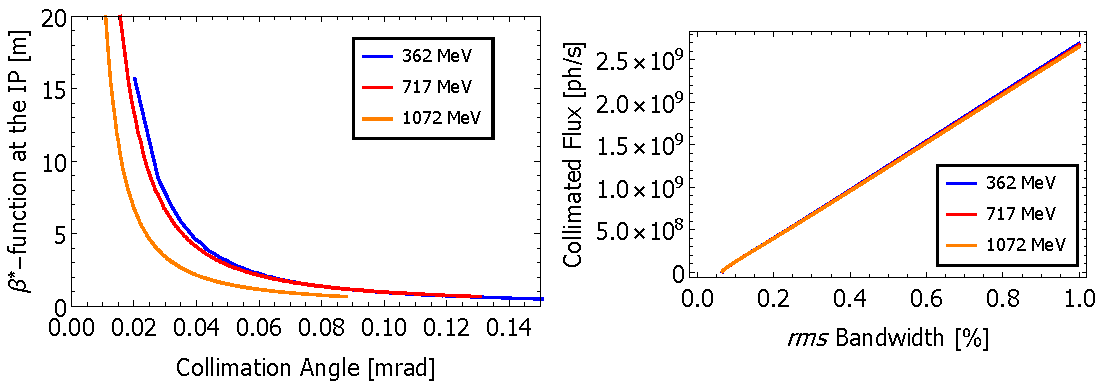
\includegraphics[width=\textwidth]{Figures/DIANA_Inverse_Compton_Source_Design/DIANA_Tuning_Curve_Opt/DIANARBplot.pdf}
\caption{Round beam optimisation comparison at the three nominal energies 362~\si{\mega\electronvolt} (blue), 717~\si{\mega\electronvolt} (red), 1072~\si{\mega\electronvolt} (orange) of the DIANA ICS source. Left: Optimised tuning curves of the $\beta^{*}$-function at the IP (same in both planes) against the collimation angle for each nominal electron energy. Right: collimated flux as a function of the \textit{rms} bandwidth of the DIANA ICS source at each nominal energy.}
\label{fig:DIANA_RB_comparison}
\end{figure}

The $\beta$-function at the IP--collimation angle parameter space tuning curves for each nominal energy in Fig~\ref{fig:DIANA_RB_comparison} each show an 'elbow' style shape, the left hand side of this plot (smaller collimation angle, larger $\beta$-function) corresponds to the narrowest bandwidth therefore smaller flux whereas the right hand side of the plot (larger collimation angle, smaller $\beta$-function) coincides with the highest flux, largest bandwidth optimisations. A difference in energy is observed between the three parameter space tuning curves in the $\beta^{*}$--$\theta_{\mathrm{col}}$ parameter which largely can be explained by the variation in $\psi=\gamma\theta_{\mathrm{col}}$ parameter that appears in the bandwidth, when $\beta^{*}$--$\psi$ is plotted there is a greater agreement between the tuning curves though remaining differences can be explained via the recoil parameter. Within the $\beta^{*}$--$\theta_{\mathrm{col}}$ tuning curve, all configurations above the line are possible with optimised configurations, in the range 0--1\% \textit{rms} bandwidth, laying on the tuning curve.   

The right hand plot of Fig~\ref{fig:DIANA_RB_comparison} shows the pareto front of the collimated flux against the \textit{rms} bandwidth according to the round beam optimisation method. The tuning curve shows the maximum collimated flux available to users within the narrowband regime when the $\beta$-functions in each plane are symmetric. We see only a small variation in the tuning curves due to electron bunch energy which is a reflection of the small variation in the magnitude of the recoil parameter between energies, for example the recoil parameters are $X_{1072~\mathrm{\si{\mega\electronvolt}}} = 0.019$ and $X_{717~\mathrm{\si{\mega\electronvolt}}} = 0.013$ for the DIANA 1072~\si{\mega\electronvolt} and 717~\si{\mega\electronvolt} cases respectively. 

\begin{figure}[!h]
\centering
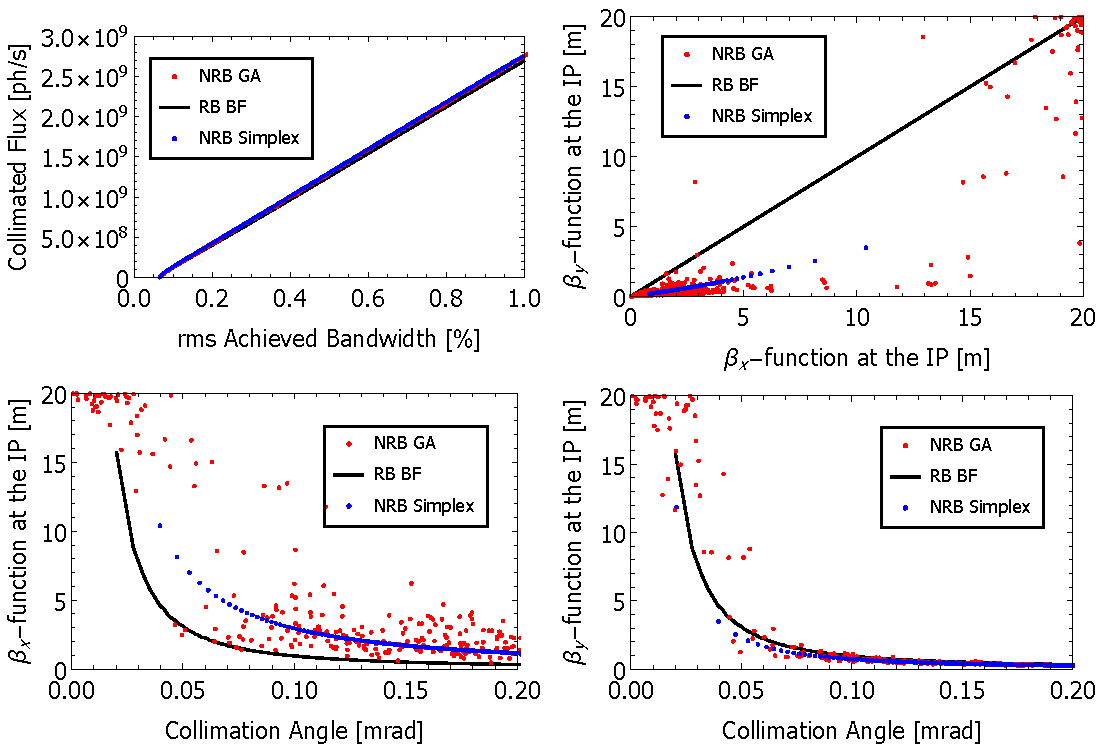
\includegraphics[width=\textwidth]{Figures/DIANA_Inverse_Compton_Source_Design/DIANA_Tuning_Curve_Opt/DIANA362fullcomp.pdf}
\caption{DIANA 362~\si{\mega\electronvolt} 1st turn ICS source optimisations, comparing the two non-round beam approaches (simplex and GA) and the round beam approach. Top Left: collimated flux as a function of \textit{rms} bandwidth pareto fronts of the source. Top Right: interaction point $\beta$-function parameter space in the $x$ and $y$ plane for optimised cases. Bottom Left: parameter space of the interaction $\beta$-function in the $x$ plane and collimation angle for optimised cases. Bottom Right: parameter space of the interaction $\beta$-function in the $y$ plane and collimation angle for optimised cases.}
\label{fig:DIANA362_comparison_optimisation}
\end{figure}

\begin{figure}[!h]
\centering
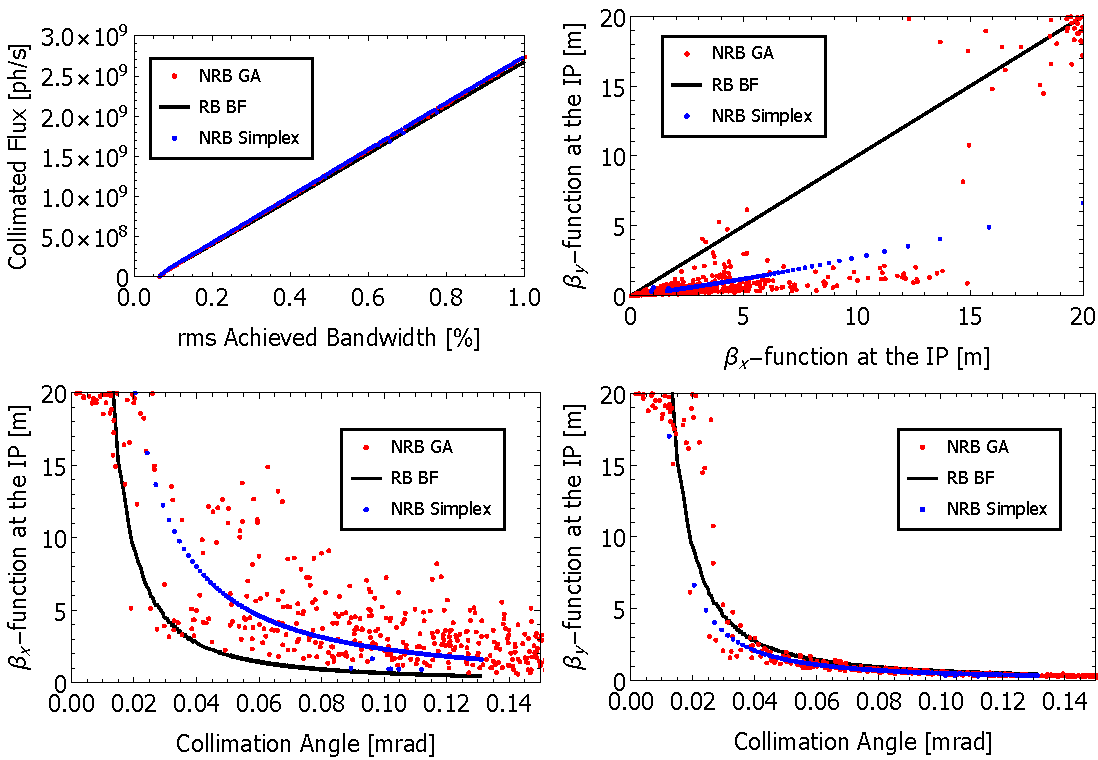
\includegraphics[width=\textwidth]{Figures/DIANA_Inverse_Compton_Source_Design/DIANA_Tuning_Curve_Opt/DIANA717fullcomp.pdf}
\caption{DIANA 717~\si{\mega\electronvolt} 2nd turn ICS source optimisations, comparing the two non-round beam approaches (simplex and GA) and the round beam approach. Top Left: collimated flux as a function of \textit{rms} bandwidth pareto fronts of the source. Top Right: interaction point $\beta$-function parameter space in the $x$ and $y$ plane for optimised cases. Bottom Left: parameter space of the interaction $\beta$-function in the $x$ plane and collimation angle for optimised cases. Bottom Right: parameter space of the interaction $\beta$-function in the $y$ plane and collimation angle for optimised cases.}
\label{fig:DIANA717_comparison_optimisation}
\end{figure}

\begin{figure}[!h]
\centering
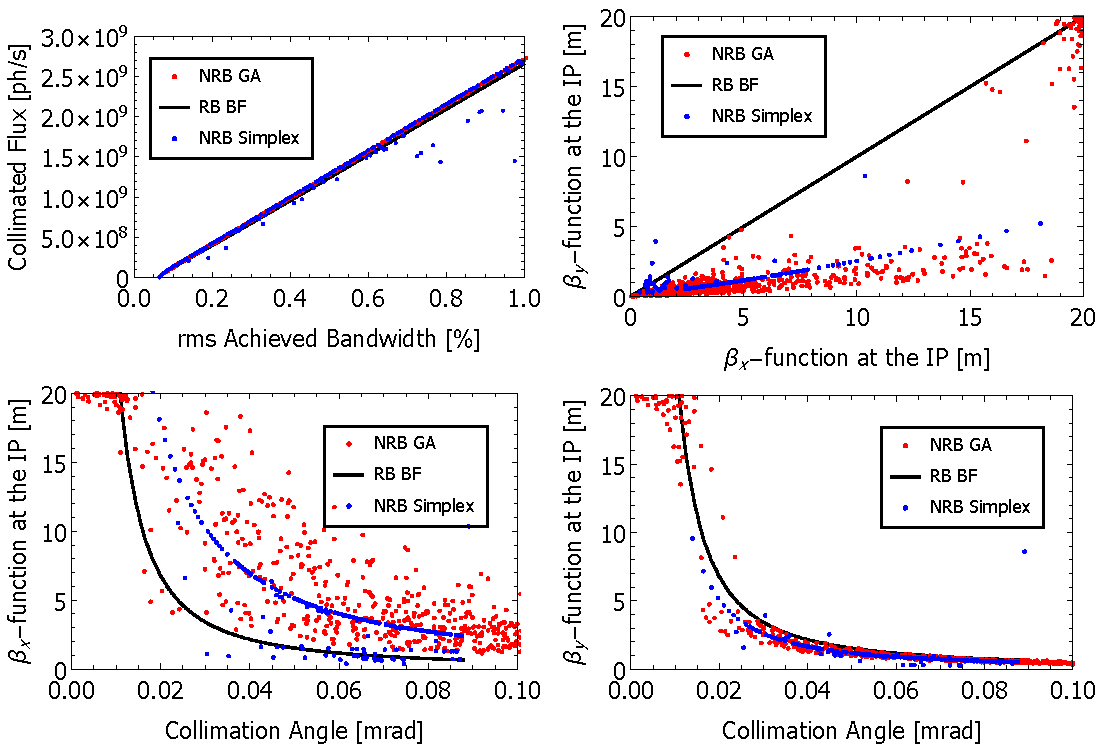
\includegraphics[width=\textwidth]{Figures/DIANA_Inverse_Compton_Source_Design/DIANA_Tuning_Curve_Opt/DIANA1072fullcomp.pdf}
\caption{DIANA 1072~\si{\mega\electronvolt} 3rd turn ICS source optimisations, comparing the two non-round beam approaches (simplex and GA) with the round beam approach. Top Left: collimated flux as a function of \textit{rms} bandwidth pareto fronts of the source. Top Right: interaction point $\beta$-function parameter space in the $x$ and $y$ plane for optimised cases. Bottom Left: parameter space of the interaction $\beta$-function in the $x$ plane and collimation angle for optimised cases. Bottom Right: parameter space of the interaction $\beta$-function in the $y$ plane and collimation angle for optimised cases.}
\label{fig:DIANA1072_comparison_optimisation}
\end{figure}



\section{$\gamma$-ray ICS Source Comparison}
\label{sec:gamma_ICS_comparison}

Inverse Compton scattering sources for production of $\gamma$-rays have been developed and designed worldwide. Differing approaches for the production of $\gamma$-rays have been trialed such as variations on the type of accelerators and incident photon sources used. For example, the HI$\gamma$S source uses radiation produced from a free electron laser to achieve high energy photon production up to 100~\si{\mega\electronvolt}. The most relevant facilities for comparison to the DIANA ICS are tabulated in Table~\ref{tab:gammaray_ICS_comparison}, this presents a combination of operating facilities and recently designed sources. 

\begin{table}[!h]
\caption{Comparison of existing and designed $\gamma$-ray ICS.}
\begin{threeparttable}
\begin{tabular}{lccc}
\hline\hline
ICS & Accelerator Type & Scattered Photon Energy (\si{\mega\electronvolt}) & Flux (ph/\si{\second}) \\
\hline
DIANA\tnote{*} & ERL & 2.33--20.11 & 5.77--6.08$\times 10^{11}$ \\ 
NIJI-IV \cite{sei2017demonstration} & Storage Ring & 1.2 & 3.1$\times 10^{4}$ \\ 
ELI-NP-GBS\tnote{*} \cite{adriani2014technical} & Linac & 0.2--19.5 & $3.9\times 10^{9}$ \\
ELI-NP VEGA\tnote{*} \cite{tanaka2020current,elinp2019vega} & Storage Ring & 1--19.5 & 1$\times 10^{11}$\\
NewSUBARU \cite{utsunomiya2015gamma} & Storage Ring & 5--40 & $3\times 10^{7}$ \\
%VELOCIRAPTOR & Linac & & \\
%T-REX & Linac & & \\
Pan et al CBS\tnote{*} \cite{pan2019design} & Storage Ring & 4--10 & 0.14--3.87$\times 10^{12}$ \\ 
Super-ACO \cite{nutarelli1998gamma} & Storage Ring & 13 & $5\times10^{6}$ \\
HI$\gamma$S\tnote{$\dagger$} ~\cite{weller2009research} & Storage Ring & 1--100 & 5$\times 10^{7}$--5$\times 10^{8}$ \\
\hline\hline
\end{tabular}
\begin{tablenotes}
\item[*]{Denotes design parameters for sources which are not yet demonstrated.}
\item[$\dagger$]{The HI$\gamma$S source is capable of scattered photon energies up to 100~\si{\mega\electronvolt}. }
\end{tablenotes}
\end{threeparttable}
\label{tab:gammaray_ICS_comparison}
\end{table}

As is evident from Table~\ref{tab:gammaray_ICS_comparison}, in-depth consideration of an ERL as the driver of an inverse Compton scattering source for production of $\gamma$-rays is limited. Predominantly ICS $\gamma$-ray production is driven by storage ring methods with the existing facilities such as NewSUBARU and HI$\gamma$S sources utilising existing synchrotron facilities. 

\section{Bremsstrahlung Source Comparison}

\section{DIANA ICS Applications}
\textcolor{blue}{**$\gamma$-ray applications from CBETA** \\ **SOME MAY BE USEFUL**}

The final ambitious application, nuclear resonance fluorescence (NRF), is a technique suitable for a future, higher-energy ERL based ICS, with an electron beam energy on the order of 350~\si{\mega\electronvolt} or above. This electron beam energy regime boosts the Compton back scattered photons into the regime of gamma rays with an energy of 2.2~\si{\mega\electronvolt} or above. These in turn would be used to excite nuclear levels identifying them with a energy sensitive solid state detector, achieving the nuclear sister spectroscopy to the atomic fluorescence spectroscopy mentioned in our first application. Such spectroscopy would be very useful in assaying nuclear materials, for example identification of manufacturing defects in fission fuel assemblies, nonproliferation security of spent fission fuel and identification of unknown legacy wastes~\cite{angal2018perle,angell2015demonstration,bolind2015states,geddes2017impact,kwan2011discrete}. Moving up to photon energies above $5$~\si{\mega\electronvolt} (requiring a \si{\giga\electronvolt}-scale electron ERL) would open up the nuclear transmutation reactions $(\gamma,p)$, $(\gamma,n)$, $(\gamma,f)$ with potentially far-reaching applications in waste transmutation \cite{ur2017optimization}, the understanding of fission dynamics \cite{bellia1983towards,bhike2017exploratory,finch2018monoenergetic} and bespoke medical isotope production from existing waste streams \cite{habs2011production}. 

\end{document}